%%%%%%%%%%%%%%%%%%%%%%%%%%%%%%%%%%%%%%%%%%%%%%%%%%%%%%%%%%%%%%%%%%%%%%%%%%%%%%%%
%2345678901234567890123456789012345678901234567890123456789012345678901234567890
%        1         2         3         4         5         6         7         8

\documentclass[letterpaper, 10 pt, conference]{ieeeconf} % Comment this line out
                                                          % if you need a4paper
                                                          % paper

\IEEEoverridecommandlockouts                              % This command is only
                                                          % needed if you want to
                                                          % use the \thanks command
\overrideIEEEmargins
% See the \addtolength command later in the file to balance the column lengths
% on the last page of the document


\title{\LARGE \bf
Robust Passivity-Based Control of Underactuated Systems via %
Neural Approximators and Bayesian Inference
}


\author{Nardos Ayele Ashenafi$^{1}$, Wankun Sirichotiyakul$^{1}$, Aykut C. Satici$^{2}$% <-this % stops a space
\thanks{$^{1}$Electrical and Computer Engineering Department
        }%
\thanks{$^{2}$Mechanical and Biomedical Engineering Department
        }%
\thanks{$^{1, 2}$Boise State University, Boise, ID 83725, USA}
}



\usepackage{algorithm2e}

\begin{document}


\maketitle
\thispagestyle{empty}
% \pagestyle{empty}

% \begin{IEEEkeywords}
%         Robotics, robust control, machine learning, nonlinear control systems
% \end{IEEEkeywords}

%%%%%%%%%%%%%%%%%%%%%%%%%%%%%%%%%%%%%%%%%%%%%%%%%%%%%%%%%%%%%%%%%%%%%%%%%%%%%%%%

\chapter*{Abstract}
\addcontentsline{toc}{chapter}{Abstract}

We provide several data-driven control design frameworks for contact-rich
robotic systems.
%
These systems exhibit continuous state flows and discrete state transitions,
which are governed by distinct equations of motion.
%
Hence, it is difficult to design a single policy that can control the system in
all modes.
%
Typically, hybrid systems are controlled by multi-modal policies, each manually
triggered based on observed states.
%
However, as the number of potential contacts increase, the number of policies
can grow exponentially and the control-switching scheme becomes too complicated
to parameterize.
%
To address this issue, we design contact-aware data-driven controllers given by
deep-net mixture of experts.
%
This architecture learns switching-control scheme that can achieve the
desired overall performance of the system, and a gating network, which
determines the region of validity of each expert, based on the observed states
%


Additionally, we address the adverse effects of model uncertainties in the
control of contact-rich robots.
%
Lack of accurate environmental models can misrepresent the effects of contact
forces on the system.
%
Policies designed from such models can lead to poor performance or even
instability.
%
In particular, we demonstrate the effects of system parameter uncertainties and 
measurement errors on the overall performance of the system.
%
Then, we design data-driven stochastic controllers that combine the stability
properties of passivity-based control with the robustness properties of Bayesian
learning.
%




\section{Introduction}

% The essence passivity-based control (PBC) paradigm is to view dynamical systems
% as subsystems that exchange energy with one another. 
% %
% The control problem is cast as a search for an interconnection pattern such that
% the overall energy function exhibits stability
% properties~\cite{ortega2001putting}.
%
Passivity-based control (PBC)~\cite{ortega2001putting,van2000l2} is a
methodology that casts the control problem as a search for an interconnection
pattern among subsystems such that the overall dynamics exhibits passivity
properties, which help infer stability.
%
The standard PBC approach in the robot control domain amounts to shaping the
system's overall energy with a fictitious one and injecting damping to
achieve asymptotic stability.
%
In practice, the closed-loop energy function is typically chosen as a quadratic
function of the error to the desired equilibrium point.
%
However, a limit of this approach is the lack of a clear connection between the
form of the desired energy function and the performance objective of a given
task.
%
Furthermore, control synthesis in PBC methods relies strongly on the dynamical
model, and imperfect compensation of the system's energy may lead to poor
performance or even instability.
%
This raises concerns regarding model uncertainties, especially in dynamical
systems with large number of parameters~\cite{nagy,wu2020active}.
%
% Although passive systems admit some inherent robustness
% properties~\cite{van2000l2}, imperfect compensation of the system's energy in
% PBC may result in instability.
%


There are techniques that combine tools from optimization, probability theory,
and machine learning to learn control strategies from inaccurate system models
or even unknown dynamics.
%
% Researchers have been tackling similar problems using a combination of tools
% from optimization, probability theory, and machine learning.
%
% Reinforcement learning (RL)~\cite{sutton2018reinforcement} uses data-driven
% techniques to find approximate solutions to the Hamilton-Jacobi-Bellman
% equation, which is the quintessential task of optimal control.
%
One example in this domain is reinforcement learning (RL), wherein the quintessential
task is to find a mapping from the observed states to the control input such
that the long-term cumulative reward is maximized.
%
Many variants of RL view the dynamical system as a black-box, which may be
represented by a real system or a simulation, and rely on repeated interactions
with the unknown environment to improve the control law.
%
One way to account for model uncertainties within this method is to perform training
directly on the real system.
%
% However, to avoid damage, training may require conservative state constraints,
% consequently limiting the capabilities of the learning
% techniques~\cite{ARGALL2009469,beaudoin2021structured}.
%
While RL methods evidently offer more flexibility on how they learn from the
unknown environment~\cite{heess2017emergence, andrychowicz2020learning,
lillicrap2015continuous}, most of them discard any potential geometric or
algebraic structures that may be useful in control synthesis.
%
This prohibitively increases the sample complexity and limits the ability to
infer stability properties.


% In contrast to black-box approaches, constructing learning frameworks based on
% prior knowledge and physical principles have been shown to be much more
% efficient~\cite{zhong2019symplectic,greydanus2019hamiltonian,sirichotiyakul2020data}.
% %
% In~\cite{zhong2019symplectic}, a learning framework for discovering Hamiltonian
% dynamics is proposed, and the controller is synthesized using passivity-based
% techniques.
% %
% We proposed in~\cite{sirichotiyakul2020data} a data-driven PBC framework where
% the desired energy function is expressed by a neural network, which is optimized
% based directly on the performance of the closed-loop trajectories of the system.
% %
% A similar approach is again explored in~\cite{massaroli2021optimal}.
% %
% However, these model-based approaches do not present a trivial solution to
% address uncertainties in the nominal dynamical model from which they are
% formulated.


Bayesian learning~\cite{gal2016improving,thakur} offers an alternative method to
simultaneously combat model uncertainties while preserving the useful physical
structure in a data-driven framework.
%
% It has already proven effective in the modeling of dynamical systems. 
%
For instance, it is used to model disturbances, such as the effect of wind gusts
on quadcopters and the motion of other vehicles in autonomous
driving~\cite{sadigh2015safe}. 
%
% Nonlinear dynamics can be decomposed into segments of linear dynamics, and learn
% the linear dynamical units and their transition probabilities through
% BL~\cite{pmlr-v54-linderman17a}. 
%
% Bayesian learning is also used in motion planning and control synthesis. 
%
In human-robot interactions, such as prosthetics and rehabilitation devices,
Bayesian neural networks can classify and predict motions in order to generate
reliable commands for the device~\cite{motionclassification}. 
% %
% Given an optimal policy, \cite{thakur} uses Bayesian neural networks to detect
% uncertainties caused by offset between training and testing conditions. When the
% uncertainty is high, the controller switches to a fallback strategy that
% requests more demonstrations. 
%
% In~\cite{lazkano2007use}, a Bayesian neural network trained using data generated
% only from sonar readings is used to generate task-execution commands for
% mobile robots.
%
% A unified learning-based approach that incorporates combines traditional control
% theory and addresses uncertainties is still missing from the literature.
%
However, the literature on applications of Bayesian learning in the control of
uncertain dynamical systems is scarce.

% {
%     \color{magenta}
%     We present a theoretical justification for the robustness properties of
%     controllers obtained from Bayesian learning techniques in~[23]. In [23],
%     we compare the performance of deterministic and Bayesian solutions to
%     the optimal control search problem for a simple dynamical system under
%     uncertainties. Our analysis shows that the deterministic solution is
%     sensitive to system parameter uncertainty and measurement noise.
%     Moreover, the Bayesian solution reasons about the stability of the
%     system under these uncertainties. In the following sections, we extend
%     the findings of [23] to a more complex control synthesis technique, such
%     as PBC.
    
% } 


In this work, we present a unified framework that simultaneously combines PBC
techniques and rigorously addresses model uncertainties using Bayesian learning.
%
{\color{magenta} The specific contributions of this work are threefold: (i)
Motivated by~\cite{sirichotiyakul2020data}, we incorporate uncertainties into
the dynamics and cast the passivity-based control synthesis problem as a
stochastic optimization problem.
%
The closed-loop storage (energy-like) function, from which the control law is
derived, is not restricted to a certain form and instead represented by a neural
network whose parameters are random variables.
%
% The second aim is to develop an algorithm that find a suitable family of
% parameters for the energy-like function such that the behavior of the
% closed-loop trajectories optimizes a certain performance objective.
%
(ii) We apply Bayesian learning and develop an algorithm that finds
a suitable probability distribution of the neural net parameters automatically.
%
In contrast to deterministic optimization, this approach provides a probability
distribution over the neural net parameters instead of a point estimate,
providing a way to reason about model uncertainties and measurement noise during
the learning process.
%
(iii) We demonstrate the efficacy and robustness of our current framework with a
comparison against our deterministic
framework~\cite{sirichotiyakul2020data}. The comparison is performed on a
benchmark underactuated control problem--the inertia wheel pendulum--both in
simulation and real-world experiments. 
}


% {
 %   \color{magenta}
    %
    % The contributions of this work are summarized as follows:
    % \begin{enumerate}
    %     % \item Without destroying the structure of the underlying physical system, we
    %     % leverage the intrinsic stability properties of the IDA-PBC method and
    %     % formulate an optimization problem that finds surrogates for the solutions to
    %     % the essential nonlinear PDEs.
    %     \item Formulate a stochastic optimization problem that addresses system parameter and measurement uncertainties and preserves the properties of PBC presented in [12],
    %     \item Solve the stochastic optimization problem via Bayesian learning techniques,
    %     \item Compare the robustness properties of the solution obtained from Bayesian learning techniques with the deterministic PBC solution from [12].
    % \end{enumerate} 
% }
% The summary of our contributions is as follows:
% %
% \begin{itemize}[label=\diamond,topsep=-\parskip+3pt, itemsep=0pt, leftmargin=0pt, itemindent=2.4\listparindent, labelsep=2pt]
%     \item \textsc{NeuralPbc}, which finds the desired energy-like
%     function that optimizes the behavior of the closed-loop trajectories
%     \item A Bayesian learning framework, which infers robustness of
%     \textsc{NeuralPbc} against model uncertainties.
%     \item Validation of our methods on the inertia wheel pendulum, a benchmark
%     underactuated control problem, both in simulation and on a real system.
% \end{itemize}



% In order to learn a robust controller in simulation, we modify our deterministic
% learning technique into a Bayesian framework. 
% %
% The development of controllers under the Bayesian framework has two main
% advantages. 
% %
% First, Bayesian learning can account for uncertainties by learning a
% probability distribution over the parameters of the controller. 
% %
% Hence, we leverage this technique to minimize the adverse effects of system
% parameter uncertainties and measurement error on the control parameters.
% % First, any deterministic data-driven learning technique can be modified into a
% % Bayesian learning framework that accounts for uncertainties by learning a
% % probability distribution over the parameters of the controller. 
% %
% % Second, Bayesian learning can improve on parameters learned from deterministic
% % learning techniques in simulation to guarantee robust performance on the real
% % system. 
% %
% Second, we can use parameters learned from deterministic learning techniques as
% priors to the Bayesian learning. 
% %
% This allows us to improve the robustness properties of the deterministic
% training without learning from scratch.
% %
% To best demonstrate these concepts, we use data-driven passivity-based-control
% (PBC) as the deterministic learning technique on which we improve.

% % This paper has two main contributions: 1) deterministic data-driven PBC
% % techniques are used to learn energy-like function of the closed-loop system
% % parameterized by a neural network, 2) a Bayesian learning framework is injected
% % into the deterministic learning scheme to learn a controller robust against
% % uncertainties created by an offset between simulation training and experimental
% % testing. 
% % %
% % The remainder of the paper is organized as follows: {\todo[inline]{ complete
% % once all sections are known}}


\section{Background}

This section provides a brief technical background on which the proposed
learning framework is based upon. 

\subsection{Passivity-Based Control}
\label{ssec:pbc}

Let $x \in \mathcal{X} \subset \mathbb{R}^{2n}$ denote the state of the robot.
%
The state $x$ is represented in terms of the generalized positions and momenta
$x = (q, p)$. 
%
With $M \succ 0$ denoting the symmetric, positive-definite mass matrix, the Hamiltonian
$H$ of the robot is expressed as 
%
\begin{equation}
    H(q,p) = \frac{1}{2} p^\top M^{-1}(q) p + V(q),
    \label{eq:system_hamiltonian}
\end{equation}
%
where $V(q)$ represents the potential energy. The system's equations of motion
can then be expressed as 
%
\begin{align}
    \begin{split}  
      \bmat{\dot{q} \\ \dot{p}} &= \bmat{0 & I_n \\ -I_n & 0}\bmat{\nabla_qH \\
      \nabla_pH} + \bmat{0 \\ G(q)}u, \\
      &\hspace{-0.15cm} y = G(q)^\top \dot{q},
    \end{split}
    \label{eq:hamiltonian_dynamics}
\end{align}
%
where $G(q) \in \mathbb{R}^{n \times m}$ is the input matrix, $I_n$ denotes the
$n \times n$ identity matrix, and $u \in \mathbb{R}^m$ is
the control input.
%
The system~\eqref{eq:hamiltonian_dynamics} is \textit{underactuated} if rank $G
= m < n$.



The main idea of passivity-based control (PBC)~\cite{van2000l2} is to design the
input $u$ with the objective of imposing a desired storage function $H_d:
\mathcal{X} \rightarrow \mathbb{R}$ on the closed-loop system, rendering it
passive and consequently stable.
%
% The standard formulation of PBC is to let the control action $u = \beta(x) + v$
% such that the closed-loop dynamics satisfies
%
In the standard formulation of PBC, the control comprises an
energy shaping term and a damping injection term:
%
\begin{equation}
  u = u_{es}(x) + u_{di}(x),
  \label{eq:ida-pbc_control}
\end{equation}
%
such that the closed loop dynamics satisfies
%
\[
  H_d(x(t)) - H_d(x(0)) = \int_0^t u_{di}^\top(\tau) y(\tau) \, \dd \tau - d^\star(x(t)),
\]
%
where $d^\star \geq 0$ is the desired damping dissipation. 
%
For mechanical systems, one solution to the PBC problem is of the form
%
\begin{align*}
  u_{es}(x) &= 
  % -\left( G^\top G  \right)^{-1} G^\top
  -G^{\dagger}
  \left( \nabla_q H_d - \nabla_q H \right), \\
  u_{di}(x) &= - K_{v} \, y,%\quad \mathbb{R}^{m \times m} \ni K_v \succ 0,
\end{align*}
%
where $G^\dagger = \left( G^\top G  \right)^{-1} G^\top$, and $K_v \succ 0$ is the
damping gain matrix. The choice for $H_d$ must satisfy
%
\[
  G^\bot \left( \nabla_q H_d - \nabla_q H \right) = 0,
\]
%
where $G^\perp G = 0$,
and $H_d$ has a minimum at the desired equilibrium $x^\star = (q^\star, 0)$. 
%
% The most straight-forward solution is to assign a
% quadratic potential energy such that the minimum is at $q^\star$, i.e., with $K_p \succ 0$,
% %
% \begin{equation}
%   H_d(q,p) = \frac{1}{2} p^\top M^{-1}(q) p + \frac{1}{2}(q - q^\star)^\top K_p (q - q^\star).
%   \label{eq:quadratic_potential}
% \end{equation}
% %
% There is, in general, an infinite number of choices for $H_d$ that achieves the
% objective of PBC. 
% %
% Control researchers have proposed several systematic methods to design a
% suitable $H_d$, leading to a variety of PBC techniques. 
% %
% Some extensions introduce additional algebraic structure to the system in order
% to improve performance and ease stability analysis for a family of dynamical
% systems.


% In the interconnection and damping assignment
% (IDA-PBC)~\cite{ortega2002stabilization}, the closed-loop dynamics to chosen to
% take on the port-controlled Hamiltonian (PCH) form:
% %
% \begin{equation}
%   \bmat{\dot{q} \\ \dot{p}}
%   =
% %   \bmat{J_d(q,p) - R_d(q,p)}
%   \bmat{0 & M^{-1}M_d \\ -M_dM^{-1} & J_2(q,p) - GK_vG^\top}
%   \bmat{\nabla_q H_d \\ \nabla_p H_d},
%   \label{eq:pch}
% \end{equation}
% %
% where $J_2 = -J_2^\top$. 
% % serves as free parameters to ease solving the required
% % PDEs~\eqref{eq:pde_main}, and $K_v \succ 0$ is the tunable gain for
% % damping injection.
% %
% The storage function $H_d$ is another Hamiltonian, which is quadratic in the
% system momenta:
% %
% \begin{equation}
%     H_d(q, p) = \frac{1}{2} p^\top M_d^{-1}(q) p + V_d(q),
%     \label{eq:desired_hamiltonian}
% \end{equation}
% %
% where $M_d(q) \succ 0$ is the closed-loop, positive definite mass matrix and
% $V_d: \mathbb{R}^n \to \mathbb{R} $ is the closed-loop potential energy function
% that satisfies
% %
% \begin{equation}
%   q^\star = \underset{q}{\textrm{argmin}} \; \; V_d(q).
%   \label{eq:argmin_Vd}
% \end{equation}
% %
% % The control law that achieves the objective of IDA-PBC comprises an
% % energy-shaping term and a damping injection term, i.e.
% % %
% % \begin{equation}
% %     u = u_{es}(q,p) + u_{di}(q,p).
% %     \label{eq:ida-pbc_control}
% % \end{equation}
% %
% The energy-shaping term of~\eqref{eq:ida-pbc_control} requires a solution to
% %
% \begin{equation}
%     Gu_{es} = \nabla_qH - M_dM^{-1} \nabla_qH_d + J_2M_d^{-1}p.
%     \label{eq:Gues}
% \end{equation}
% %
% If system is underactuated, $G$ is not invertible, and Equation~\eqref{eq:Gues}
% cannot be uniquely solved. This leads to the constraints that must be satisfied
% for any choice of $u_{es}$:
% %
% \begin{equation}
%   G^\perp \left\{ \nabla_qH - M_dM^{-1} \nabla_qH_d + J_2M_d^{-1}p \right\} = 0.
%   \label{eq:pde_main}
% \end{equation}
% %
% Equation~\eqref{eq:pde_main} is a set of nonlinear partial differential
% equations (PDE) parametrized by $M_d$, $V_d$, and $J_2$. 
% %
% The skew-symmetric matrix $J_2$ serves as free parameters to ease obtaining a
% solution to~\eqref{eq:pde_main}.
% %
% The success of the IDA-PBC approach hinges on the ability to solve this set of
% PDEs.
% %
% Once a solution is obtained, the energy shaping term of the control is
% %
% \begin{equation}
%   u_{es} = G^{\dagger} \left(\nabla_qH - M_dM^{-1} \nabla_qH_d + J_2M_d^{-1}p\right),
%   \label{eq:ues}
% \end{equation}
% %
% where $G^{\dagger} = \left(G^\top G\right)^{-1} G^\top$.
% %
% With $K_v \succ 0$ a user-selected gain matrix, the damping injection term is given as
% %
% \begin{equation}
%     u_{di} = -K_v G^\top \nabla_p H_d.
%     \label{eq:udi}
% \end{equation}

% \begin{prop}
%   The closed-loop Hamiltonian $H_d$ in IDA-PBC is, by construction, a Lyapunov
%   function for the closed-loop system. The time-derivative of $H_d$ is
%   \begin{align*}
%       \dot{H}_d 
%       &= \left( \nabla_{q} H_d \right)^\top \dot{q} + \left( \nabla_p H_d \right)^\top \dot{p} \\
%       &= -\left( \nabla_{p} H_d \right)^\top \left(J_2 - G K_v G^\top\right) \nabla_p H_d \\
%       &\leq -\lambda_{\textrm{min}} \{ K_v \} \abs{ \left( \nabla_p H_d \right)^\top G }^2 \leq 0,
%   \end{align*}
%   where the last inequality follows from $J_2 = -J_2^\top$ and $K_v \succ 0$.
%   Therefore, as long as $V_d$ is bounded from below and the
%   conditions~\eqref{eq:argmin_Vd} and~\eqref{eq:pde_main} are satisfied,
%   $(q^\star, 0)$ is a stable equilibrium of~\eqref{eq:pch}.
%   \label{prop:lyapunov}
% \end{prop}


Controllers designed using PBC techniques are based on a nominal
dynamical model~\eqref{eq:hamiltonian_dynamics}. 
%
For many applications, the uncertainties in system parameters are not
negligible. 
%
In this work, we attempt to improve the controller's robustness properties by
means of Bayesian inference, whose theory we briefly summarize in the following
subsection.


\subsection{Bayesian Inference}
\label{ssec:bays}

The objective of Bayesian learning is to generate a stochastic model that best
fits observed data. Let this stochastic model be represented by $m(x; \theta)$,
where $\theta$ is a multivariate random variable that parametrizes the model and
$x$ is the input. Given prior belief on the distribution of the parameters
$p(\theta)$, Bayesian learning finds a posterior distribution $p(\theta \mid
\mathbb{D})$ over $\theta$ that maximizes the likelihood of the model matching
the underlying source of the dataset~\cite{bishop2006pattern}. 


Bayesian learning provides various techniques to find the posterior distribution
over $\theta$, one of which is the Markov Chain Monte Carlo (MCMC) methods. MCMC
methods learn the exact posterior distribution by collecting samples of $\theta$
either through a random walk (e.g. Metropolis-Hastings) or by following the
gradient of the likelihood (e.g. Hamiltonian Monte Carlo). Unfortunately, MCMC
techniques have weak convergence properties for high-dimensional parameters.
Hence, we leverage variational inference (VI), a technique that approximates the
posterior $p(x \mid \theta)$ with the distribution $q(\theta;z)$ selected from
the conjugate family of the prior~\cite{cohen2016bayesian}.
%
% selects a specific form $q(\theta;z)$ for the posterior distribution and
% learns the distribution parameters $z$. 
%
This gradient-based method selects the distribution parameters $z$ of the
approximate posterior $q$ that maximize the evidence lower bound (\textsc{Elbo}),
$\mathcal{L}(x, z)$:
\begin{align}
  \begin{split}
  \mathcal{L}(x,z) &= \mathbb{E}_{\theta \sim q} \left[\log(p(x, \theta;z)) - \log(q(\theta;z)) \right], \\
  p(x, \theta;z) &= p(x \mid \theta;z)p(\theta),
  \end{split}
  \label{eq:elbo}
\end{align}
where $p(x \mid \theta;z)$ is the likelihood function. 

%
% The power of Bayesian learning lies in its
% ability to build a model and make predictions that integrate over
% uncertainties~\cite{tipping2003bayesian}. These predictions can be found by
% marginalizing the model over the posterior~\cite{jospin2020hands}.
% \begin{equation}
%   \hat{m} = \frac{1}{N} \sum_{\theta \sim q} m(x, \theta),
%   \label{eqn:marginalization}
% \end{equation} 
% where $N$ is the number of samples drawn from the posterior. 
%
% Moreover, Bayesian frameworks can quantify how confident we are in the model
% predictions through the variance of the predictive distribution, $p(m \mid x,
% \mathbb{D})$. 
%
% The variance of $p(m|x, \mathbb{D})$ is given
% by~\cite{jospin2020hands}
% \begin{equation}
%   \Sigma_{m \mid x,\mathbb{D}} = \frac{1}{N-1} \sum_{\theta \sim q} \vectornorm{m(x,\theta) - \frac{1}{N} \sum_{\theta \sim q} m(x, \theta)}^2.
%   \label{eqn:predictive_variance}
% \end{equation}
%

% Unlike deterministic models, whose parameters are given by point estimates,
% Bayesian learning can characterize the uncertainties in the prediction.

% %
% Deterministic model are parameterized by point estimates. Their predictions find
% an average estimate over the noisy dataset. On the other hand, Bayesian learning
% provided models that make stochastic predictions that reflect the uncertainties
% in the dataset. 


% The power of Bayesian learning lies in its ability to build a model and make
% predictions that integrate over uncertainties~\cite{tipping2003bayesian}. These
% predictions can be found by marginalizing the model over the
% posterior~\cite{jospin2020hands}.

%
Bayesian learning techniques can be made more powerful when combined with the
expressive power of Bayesian neural networks (BNN), whose weights and biases are
samples drawn from a posterior distribution~\cite{jospin2020hands}. The BNN
architecture comes with many advantages; unlike deterministic neural networks,
it can provide a model and characterize the uncertainty of predictions with a
small amount of data. The use of prior distribution also behaves like a
regularization term that prevents the model from overfitting to the training
data~\cite{tipping2003bayesian}. On the flip side, it is more complicated and
computationally expensive to learn probability distributions than point
estimates.

                           

\section{Neural Bayesian Learning}
\frame{Neural Bayesian Learning (NBL): \\
Robust Data-Driven Stochastic Control Design}

\begin{frame}[fragile]{Completed Work}

  \begin{columns}
    \begin{column}{0.58\linewidth}
      \begin{exampleblock}{Neural Bayesian Learning}
        \begin{equation*}
          \begin{aligned}
              \underset{q(\theta) }{\text{min}} 
              &&\quad J(&\phi(t; x_0, u), u) \\
              \text{subject to} 
              &&\quad \dd {x} &= f(x, u; \zeta) \dd t + \nabla_x u(x) \dd W_t, \\
              &&\quad u(x; \theta) &= \mathcal{D} \{F(x; \theta) \}, \\
              &&\quad \zeta &\sim \mathcal{N}(\zeta_0, \Sigma_\zeta), \\
              &&\quad \theta &\sim q(\theta).
          \end{aligned}    
        \end{equation*}
      \end{exampleblock}
      \begin{itemize}
        \item $F(x;\theta)$ is a \textit{Bayesian neural network}.
        \item $\phi(t;x_0, u)$ is a trajectory generated from policy $u$ starting at initial state $x_0$.
        \item $\zeta$ is a vector of system parameters with uncertainties $\Sigma_\zeta$.
        % \item The closed-form solution to the optimization problem is intractable.
      \end{itemize}
    \end{column}
    \begin{column}{0.42\linewidth}
      \centering
      % ~
      \resizebox{0.7\textwidth}{!}{%
      \begin{tikzpicture}[
        shorten >=1pt,->,draw=black!70, node distance=\layersep,
        neuron/.style={circle,fill=black!25,minimum size=20,inner sep=0},
        edge/.style 2 args={pos={(mod(#1+#2,2)+1)*0.33}, font=\tiny},
        distro/.style 2 args={
            edge={#1}{#2}, node contents={}, minimum size=0.6cm, path picture={\draw[double=orange,white,thick,double distance=1pt,shorten >=0pt] plot[variable=\t,domain=-1:1,samples=51] ({\t},{0.2*exp(-100*(\t-0.05*(#1-1))^2 - 3*\t*#2))});}
        },
        weight/.style 2 args={
            edge={#1}{#2}, node contents={\pgfmathparse{0.35*#1-#2*0.15}\pgfmathprintnumber[fixed]{\pgfmathresult}}, fill=white, inner sep=2pt
        }
      ]
        \nn{regular}
        % Draw weights for all regular edges.    
        \foreach \i in {1,...,2}
            \foreach \j in {1,...,4}
                \path (i\i-regular) -- (h\j-regular) node[weight={\i}{\j}];
        \foreach \i in {1,...,4}
            \path (h\i-regular) -- (o-regular) node[weight={\i}{1}];
    
      \end{tikzpicture}
      }

      ~

      \resizebox{0.7\textwidth}{!}{%
      \begin{tikzpicture}[
        shorten >=1pt,->,draw=black!70, node distance=\layersep,
        neuron/.style={circle,fill=black!25,minimum size=20,inner sep=0},
        edge/.style 2 args={pos={(mod(#1+#2,2)+1)*0.33}, font=\tiny},
        distro/.style 2 args={
            edge={#1}{#2}, node contents={}, minimum size=0.6cm, path picture={\draw[double=orange,white,thick,double distance=1pt,shorten >=0pt] plot[variable=\t,domain=-1:1,samples=51] ({\t},{0.2*exp(-100*(\t-0.05*(#1-1))^2 - 3*\t*#2))});}
        },
        weight/.style 2 args={
            edge={#1}{#2}, node contents={\pgfmathparse{0.35*#1-#2*0.15}\pgfmathprintnumber[fixed]{\pgfmathresult}}, fill=white, inner sep=2pt
        }
      ]
        \nn{bayes}
        % Draw distros for all Bayesian edges.
        \foreach \i in {1,...,2}
            \foreach \j in {1,...,4}
                \path (i\i-bayes) -- (h\j-bayes) node[distro={\i}{\j}];
        \foreach \i in {1,...,4}
            \path (h\i-bayes) -- (o-bayes) node[distro={\i}{1}];
      \end{tikzpicture}
      }
    \end{column}
  \end{columns}

\end{frame}


\begin{frame}{}
  \begin{algorithm}[H]
    \centering
    \small
    % \setstretch{1.0}
    \caption{Neural Bayesian Learning}
    \begin{algorithmic}
      \algrenewcommand\algorithmicindent{0em} % No indent
      \onslide<1->{
        \color{gray}
        \only<1>{\color{black}}

        \State Select a prior distribution $p(\theta)$
        \State $f \,\gets f(x, u^\theta; \zeta)$ dynamics given by SDE using current policy $u^\theta$
        \State $\mathcal{D} \gets \{x_0\}_{(N_{\mathcal{D}})}$  \Comment{$N_{\mathcal{D}}$ samples of $x_0$}
      }
      
      \algrenewcommand\algorithmicindent{1.5em} % Change indent back to default

      \onslide<1->{
        \color{gray}
        \only<2>{\color{black}}
        \For{$i=1:\texttt{maxiters}$}
          \For{each $d$ $\subset \mathcal {D}$} \Comment Select batch $d$ from dataset $\mathcal{D}$
              \State Initialize $\mathcal{J} = 0$
              \State $\theta \sim  q(\theta ; z)$ \Comment{Sample parameters of $F$ from posterior}
      }

      \onslide<1->{
        \color{gray}
        \only<3>{\color{black}}

        \For{each $x_0 \in d$}
            \State $\zeta \sim \mathcal{N}(\zeta_0,\Sigma_{\zeta})$ \Comment{Sample system parameters}
            \State $\phi(t; x_0, u^\theta) \gets$ integrate dynamics from $x_0$ 
            \State $\mathcal{J} \gets \mathcal{J} + J(\phi(t; x_0, u^\theta), u^\theta)$
        \EndFor
        \State Compose likelihood $p(d | \theta)$
        \State Compute \textsc{Elbo} $\mathcal{L}(J,z) = \mathbb{E}_{\theta \sim q} \left[\log( p(J \mid \theta;z)p(\theta;z)) - \log(q(\theta;z)) \right]$
        \State $z \leftarrow  z + \alpha \; \partial \mathcal{L} / \partial z$
        \EndFor
      }

      \onslide<1->{
        \color{gray}
        \only<4>{\color{black}}
        \State $\mathcal{D} \gets \{\mathcal{D}\}_{(1,\ldots,N_{\mathcal{D}}-N_{\textrm{R}})} \cup \{x_0\}_{(N_{\textrm{R}})}$\Comment{Replay buffer}
      \EndFor
      
      \State \textbf{return} $q(\theta; z)$
      }
    \end{algorithmic}
    \addtocounter{algorithm}{-1}
  \end{algorithm}
\end{frame}

% \begin{frame}{Gradient of \textsc{Elbo}}
%   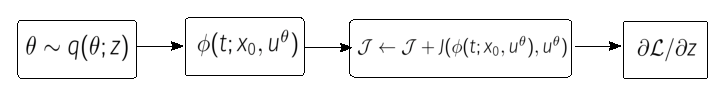
\includegraphics[width = 0.9\linewidth]{gradient.eps}
%   \begin{itemize}
%     \item Automatic differentiation techniques are used to compute gradients through the stochastic differential equations.
%   \end{itemize}
% \end{frame}

\section{Case Study: Inertia-Wheel Pendulum}
\label{sec:iwp}

In this section, we validate the proposed control design framework on the
problem of swinging-up and stabilizing the inverted position of an inertia wheel
pendulum (IWP), shown in Fig.~\ref{fig:iwp}. We provide experimental results
from simulation and real-world hardware in order to thoroughly demonstrate the
efficacy and robustness claims of Bayesian inference. 
%
We use the deterministic solution for \textsc{NeuralPbc} as the baseline
on which we compare the performance of the Bayesian solution.


\subsection{System Model}
\label{ssec:model}

The IWP mechanism consists of a pendulum with an actuated wheel instead of a static
mass.
%
The wheel has mass $m$, which is connected to a massless rod of length \(l\). 
%
The position of the rod is denoted by the angle \(q_1\) measured with
respect to the downward vertical position.
%
The position of the wheel \(q_2\) is measured with respect to the vertical
line through the center of the wheel.

The Hamiltonian of the IWP is given by Equation ~\eqref{eq:system_hamiltonian}
with $n=2$ and
%
\begin{equation*}
    M = \bmat{I_1 & 0 \\ 0 & I_2},
    \;
    G = \bmat{-1 \\ \phantom{-}1},
    \;
    V(q) = mgl \left( \cos q_1 - 1 \right),
\end{equation*}
%
and $p = \left(I_1 \dot{q}_1,I_2 \dot{q}_2\right)$. 
%
We denote the state of the system as $x = (q_1, q_2, \dot{q}_1, \dot{q}_2)$.
%
The parameters \(I_1\) and \(I_2\) denote the moment of inertia of the pendulum
and the wheel, respectively, and \(g\) is the gravitational constant.
%
% The wheel has mass $m$, which is connected to a massless rod of length \(l\). 
%
The equations of motion of the IWP can be written as 
%
\begin{equation}
    % \begin{aligned}
    %     I_1\ddot{\theta}_1 &= -mgl \sin(\theta_1) - u, \\
    %     I_2\ddot{\theta}_2 &= u
    % \end{aligned}
    % \bmat{I_1 & 0 \\ 0 & I_2} \bmat{q_1 \\ q_2} + \bmat{-mgl \sin q_1 \\ 0} = \bmat{-1 \\ \phantom{-}1} u, 
    M \bmat{\ddot{q}_1 \\ \ddot{q}_2} + \bmat{-mgl \sin q_1 \\ 0} = Gu, 
    \label{eq:iwp_dynamics}
\end{equation}
%
where the control input \(u\) is the torque applied to the inertia wheel.
%
The desired equilibrium $x^\star = (q^\star, 0)$ is the origin, which
corresponds to the upward position.
%
The nominal system parameters are estimated to be $I_1 = 0.0455$ kg-m$^2$, $I_2
= 0.00425$ kg-m$^2$, and $mgl = 1.795$ N-m. 
%
% The control objective is to ensure that closed-loop trajectories
% of~\eqref{eq:iwp_dynamics} passes through a neighborhood of $x^\star$,
% at which point a linear stabilizing controller can be employed to asymptotically
% stabilize the system at $x^\star$.
%

\begin{figure}[t]
    \centering
    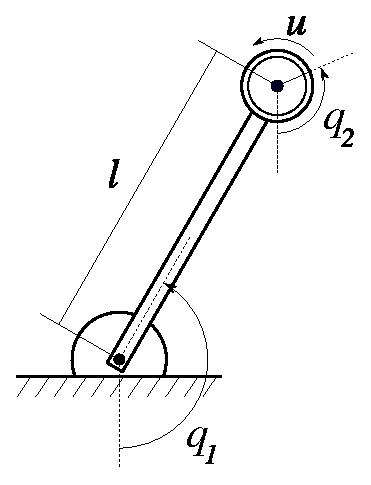
\includegraphics[width=0.25\linewidth]{figures/iwp.eps}
    \caption{Schematic of the inertia wheel pendulum. Only the joint $q_2$ is actuated, and $q_1$ is not.}
    \label{fig:iwp}
\end{figure}

% The joint $q_2$ in our hardware implementation is actuated by a Nanotec DFA90
% brushless DC motor through a belt drive system.
% %
% The motor is mounted concentrically with the joint $q_1$ to minimize $mgl$. 
% %
% The actuator torque (current) is controlled by Maxon EPOS2 70/10. 
% %
% The nominal system parameters are estimated to be $I_1 = 0.0455$ kg-m$^2$, $I_2
% = 0.00425$ kg-m$^2$, and $mgl = 1.795$ N-m. 


\subsection{Case Study}

We begin by demonstrating the \textsc{NeuralPbc} framework outlined in
Section~\ref{ssec:ml-pbc} on the IWP system. 
%
In this setting, the surrogate $H_d^\theta$ for the closed-loop energy function
is determined by solving the optimization
problem~\eqref{eq:neural_pbc_finite_optim}, and the corresponding control law is
applied on the system given by~\eqref{eq:iwp_dynamics}.
%
We apply this control law in conjunction with the Linear Quadratic Regulator
(LQR), the latter of which is activated when the trajectories enter a
neighborhood of $x^\star$.
%
Two case studies are performed: 1) solving~\eqref{eq:neural_pbc_finite_optim}
through stochastic gradient descent (deterministic training from
Section~\ref{sssec:ml-pbc-deterministic}), and 2)
solving~\eqref{eq:neural_pbc_finite_optim} through Bayesian learning
(Section~\ref{sssec:ml-pbc-bayes}).
%
The results from both case studies are compared to showcase the effectiveness of
\textsc{NeuralPbc} and the robustness benefits of Bayesian learning.


\subsubsection{Training Setup}

The energy-like function $H_d^\theta$ is a fully-connected neural network with
two hidden layers, each with the \textsc{Elu} activation function. 
%
% There are, in total, 137 parameters to learn. 
% %
% They are initialized according to the Glorot
% (Xavier)~\cite{glorot2010understanding} scheme.
%
% The objective of the optimization problem~\eqref{eq:neural_pbc_finite_optim}
% consists of $\ell_{\textrm{set}}$ given by Equation~\eqref{eq:set_distance},
% with the set $\mathcal{S}$ chosen as a ball of radius $r = 0.01$ around
% $x^\star$ in the standard norm topology.
%
A uniform distribution in $[-2\pi, 2\pi] \times [-2\pi, 2\pi] \times [-10, 10]
\times [-10, 10]$ is chosen as the probability distribution from which samples
of initial states $x_0$ are drawn for the \textsc{DAgger} strategy.
%
In each gradient descent step, a batch of 4 initial states $\{x_0\}$,
generated by the state sampling technique in~\ref{sssec:ml-pbc-sampling}, are
integrated forward with a time horizon of $t \in [0,3]$ seconds. 
%
In the Bayesian framework, the standard deviations $\sigma_{\zeta}$ of system
parameters $\zeta = [I_1, I_2, mgl]$ are chosen to be $10\%$ of the nominal system
parameters given in Section~\ref{ssec:model}.
%
Moreover, we train on trajectories per the SDE in~\eqref{eq:sde_initial} with
measurement error represented by Wiener process with standard deviation of 0.001
and 0.02 on the joint angles and velocities, respectively.
%
% In each gradient descent step, a batch of 4 initial conditions $\{x_0\}$
% generated by \textsc{DAgger} is integrated forward with using the Tsitouras
% $5(4)$ Runge-Kutta solver with a time horizon of $t \in [0,3]$ seconds. 
%
% The cost function is then computed and back-propagated using the
% AD-assisted adjoint method implemented in
% \verb|DiffEqFlux.jl|~\cite{DBLP:journals/corr/abs-2001-04385}.
% %
% In the Bayesian learning framework, we draw samples from the posterior and
% back-propagate through the gradients of the \textsc{Elbo} using the
% \textsc{ADVI}~\cite{kucukelbir2015automatic} scheme provided in
% \verb|Turing.jl|~\cite{turing}. 
%
The trainings are terminated when the loss function $\ell$ and the \textsc{Elbo}
converge for the deterministic and Bayesian trainings, respectively.
%
The hyperparameters for the deterministic and Bayesian \textsc{NeuralPbc}
trainings are shown in Table~\ref{tab:training_setup_neuralpbc}.
%
It can be seen that the Bayesian training effectively learns with smaller neural
network size and fewer data than the deterministic training.
\begin{table}[tb]
    \centering
    \caption{\textsc{NeuralPbc} training setup for deterministic and Bayesian frameworks}
    % \rowcolors{2}{}{Wheat1}
    \begin{tabular}{lcc}
      \toprule
    %   & \multicolumn{2}{c}{Framework} \\
    %   \cmidrule(lr){2-3}
       & Deterministic & Bayesian \\
      \midrule
        $H_d$ neural net size & (6, 12, 3, 1) & (6, 5, 3, 1)\\
        Learned parameters & 133 & 128  \\
        Optimizer & \textsc{ADAM} & DecayedAdaGrad\\
        Initial learning rate & 0.001 & 0.01\\
        Replay buffer size & 400 & 50\\
      \bottomrule
    \end{tabular}
    \label{tab:training_setup_neuralpbc}
  \end{table}

\subsubsection{Simulated Experiments}

%
The performance of the controllers obtained from the deterministic and Bayesian
trainings are compared as follows.
%
% Both frameworks are trained with the nominal system parameters given in
% Section~\ref{ssec:model}.
%
We evaluate the performance of both trainings with parameter uncertainties
on $I_1, I_2$ and $mgl$. 
%
We introduce these uncertainties by moving the average
system parameters by $\pm 10\%$ to $\pm 50\%$ with increments of $10\%$. 
%
For each average system parameter, we sample uniformly with a $\pm 5\%$ support
around the average system parameters. 
%
This helps test the performance of the controller with various combinations of
$I_1, I_2$ and $mgl$.
%
On top of the system parameter uncertainties, we introduce measurement noise
represented by a Wiener process with standard deviation of $0.001$ and $0.02$ on
the joint angles and velocities, respectively. 
%
Fig.~\ref{fig:comparison_neuralpbc} shows the performance of deterministic and
Bayesian trainings using an accumulated quadratic loss of the form
\begin{equation} J_T = \frac{1}{2}\int_0^T \left(x^\top Qx + u^\top Ru \right) dt.
  \label{eq:performance_metric} \end{equation}
%
The controller derived from the Bayesian training is marginalized over 10
parameters sampled from the posterior distribution. 
%
As shown in Fig.~\ref{fig:comparison_neuralpbc}, the Bayesian training
effectively incurs less cost for large error in system parameters.
%
Moreover, the error band on the cost of the Bayesian training is smaller than
that of the deterministic training, demonstrating that the marginalized
controller is more robust against measurement noise.
%   
\begin{figure}[tb]
    \centering
    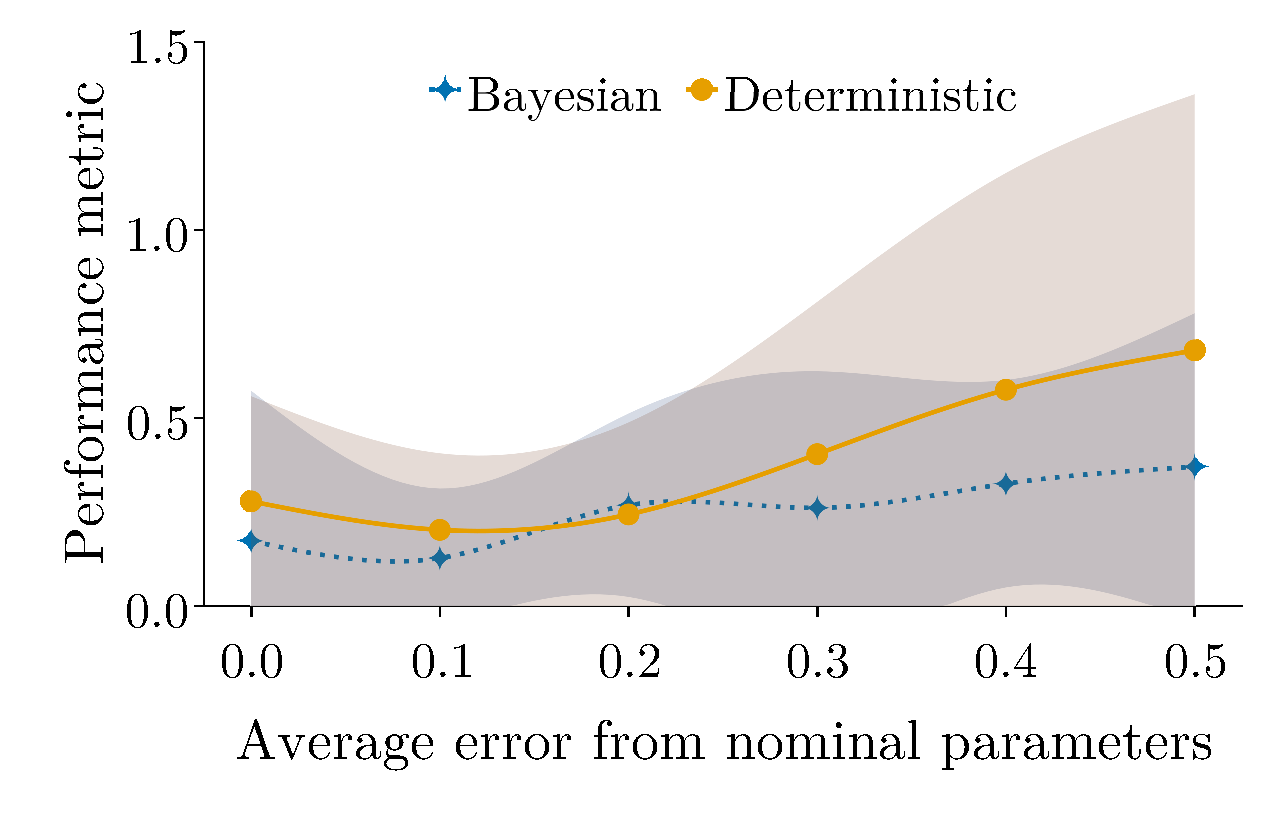
\includegraphics[clip,width=0.8\columnwidth]{./figures/bandplot2.eps}%
    \caption{\textsc{NeuralPbc} Performance metric ($J_T$) for various
    error in system parameters. Measurement noise included as Wiener process
    with standard deviation of $0.001$ and $0.02$ on joint angles and
    velocities, respectively}
    \label{fig:comparison_neuralpbc}
\end{figure}


\subsubsection{Real-World Experiments}

The controllers from both training schemes are evaluated on hardware. 
%
Since the nominal model~\eqref{eq:iwp_dynamics} neglects the friction in the
bearings any contribution to the dynamics by the belt-drive system, the hardware
experiments empirically demonstrate the robustness of our controllers against
these uncertainties.
%
We further bolster this claim by deliberately modifying the hardware and test
the controllers without any additional training.
%
In particular, throughout the experiments, the inertia wheel attached to $q_2$
is replaced with parts (labelled A-C on Table~\ref{tab:modified_params}) whose
mass and inertia are different from the nominal values.
%
The modified system parameters are summarized in
Table~\ref{tab:modified_params}.
%
% The parameter error listed on the last column of Table~\ref{tab:modified_params}
% is computed by $\|p - p_{\textrm{nom}}\| / \|p_{\textrm{nom}}\|$.
\begin{table}[tb]
  \centering
  \caption{System parameters used in real-world experiments. The errors in the
  last column are $\|p_s - p^{\textrm{nom}}_{s}\| / \|p^{\textrm{nom}}_{s}\|$}.
  % \rowcolors{2}{}{Wheat1}
  \begin{tabular}{lcccc}
    \toprule
    Parameter set $p_s$ & $I_1$ & $I_2$ & $mgl$ & Error \\
    \midrule
    Nominal & 0.0455 & 0.00425 & 1.795 & 0 \\
    A & 0.0417 & 0.00330 & 1.577 & $0.122$ \\
    B & 0.0378 & 0.00235 & 1.358 & $0.243$ \\
    C & 0.0340 & 0.00141 & 1.140 & $0.365$ \\
    \bottomrule
  \end{tabular}
  \label{tab:modified_params}
\end{table}
 
The system starts from rest at the downward position. 
%
A small disturbance in the $q_1$ direction is introduced to start the swing-up.
%
The state $x$ is recorded and~\eqref{eq:performance_metric} is the performance
metric used to evaluate the controllers.
%
% \begin{equation}
%     J_{\textrm{exp}}(x,u) = \frac{1}{2} \int_{0}^{T} 2 \bigl(1 - \cos q_1\bigr) + \dot{q}_1^2  + \dot{q}_2^2 + u^2 \, \dd t,
%     \label{eq:experiment_performance_metric}
% \end{equation}
%
% where $T$ is the time at which the switch to LQR occurs.
%
The results are summarized in Fig.~\ref{fig:neuralpbc_bar_plot}.


In all scenarios, our controllers are able to achieve the control objective
despite the errors introduced in the system parameters.
%
% Furthermore, the controller from Bayesian training consistently outperforms the
% controller from deterministic training, supporting the theoretical justification
% discussed in Section~\ref{ssec:justification}. 
%
These results demonstrate that our approach enables a unified way to tackle
nonlinear control problems while simultaneously incorporating prior knowledge
and model uncertainties.
%
\begin{figure}[t]
    \centering
    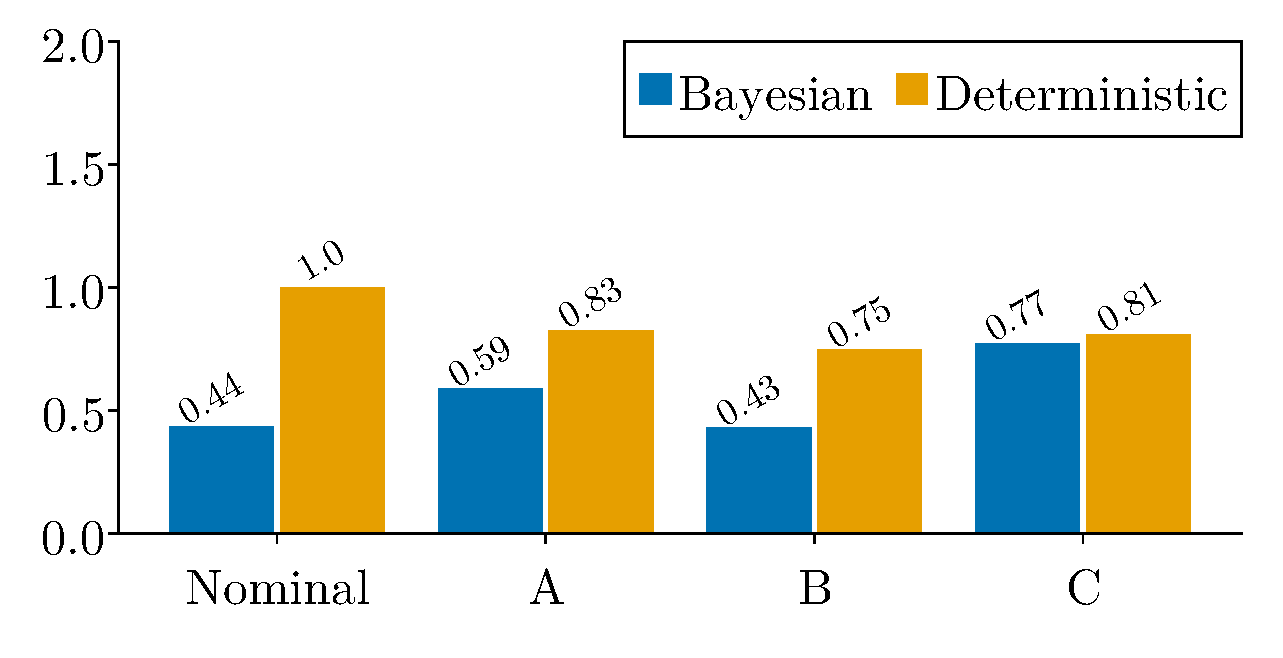
\includegraphics[width=0.9\linewidth]{pbc_bar.eps}
    \caption{
        %
        Controller performance for modified system parameters. 
        %
        The performance metric is given by
        Eq.~\eqref{eq:performance_metric}.
        %
        Lower values are better. 
        %
        These results show that controllers trained via Bayesian learning are
        consistently more robust to errors in system parameters.
        %
    }
    \label{fig:neuralpbc_bar_plot}
\end{figure}


% \begin{table}[t]
%     \centering
%     \caption{Comparison of the approaches}
%     \rowcolors{4}{}{Wheat1}
%     \begin{tabular}{lcc}
%       \toprule
%       & \multicolumn{2}{c}{Methods implemented} \\
%       \cmidrule(lr){2-3}
%       Case & Deterministic & Bayesian \\
%       \midrule
%       Robustness & \textcolor{red!88!green}{\xmark} & \textcolor{green!63!blue}{\cmark} \\
%       Computation cost & \textcolor{green!63!blue}{\cmark} &  \textcolor{red!88!green}{\xmark} \\
%       Model selection &  \textcolor{red!88!green}{\xmark} & \textcolor{green!63!blue}{\cmark} \\
%       Amount of data &  \textcolor{red!88!green}{\xmark} & \textcolor{green!63!blue}{\cmark} \\
%       Prior knowledge & \textcolor{green!63!blue}{\cmark} & \textcolor{green!63!blue}{\cmark}\textcolor{green!63!blue}{\cmark} \\
%       Learning stability & \textcolor{green!63!blue}{\cmark} &  \textcolor{red!88!green}{\xmark} \\
%       Overfitting &  \textcolor{red!88!green}{\xmark} & \textcolor{green!63!blue}{\cmark} \\
%       \bottomrule
%     \end{tabular}
%     \label{tab:comparison}
%   \end{table}

% \begin{minipage}{\textwidth}
%     \begin{minipage}[b]{0.45\textwidth}
%       \centering
%       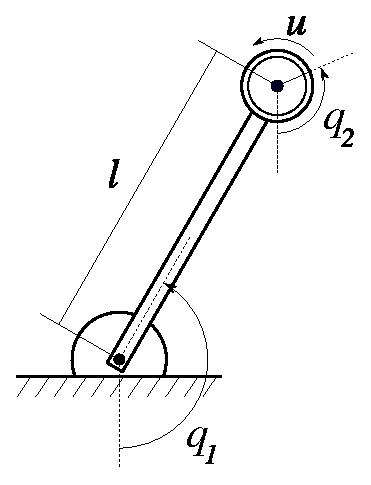
\includegraphics[width=0.5\textwidth]{figures/iwp.eps}
%       \captionof{figure}{Schematic of the inertia wheel pendulum. Only the rotating wheel \(\theta_2\) is actuated.}
%       \label{fig:iwp}
%     \end{minipage}
%     \hfill
%     \begin{minipage}[b]{0.45\textwidth}
%       \centering
%       \begin{tabular}{cc}\hline
%         Table head & Table head \\ \hline
%           Some values & Some values \\
%           Some values & Some values \\
%           Some values & Some values \\
%           Some values & Some values \\
%           Some values & Some values \\
%           Some values & Some values \\ \hline
%         \end{tabular}
%         \captionof{table}{A table beside a figure}
%         \label{tab:iwp_params}
%     \end{minipage}
% \end{minipage}

\subsection{Discussion}
\label{ssec:discussion}

Given a fixed amount of data available during a training session, the
deterministic framework has the upper hand since the Bayesian framework needs to
learn a whole probability distribution as opposed to a point summary of this
whole distribution. However, given a trustworthy prior distribution, Bayesian
framework needs much fewer data to come up with solutions that perform well. The
Bayesian framework is inherently more robust against parameter uncertainties and
measurement errors as long as the controller is computed by marginalizing the
probability distribution over the weights of the neural network as this process
is less prone to overfitting. Moreover, the Bayesian framework allows for
further training of the controller by updating the neural net parameters online;
that is, during the operation of the real system by treating the probability
distributions learned during simulation as priors.
\section{Conclusion}
\label{sec:moe_conclusion}

In this chapter, we provide a data-driven control design that reasons about the
effects of contact forces on the hybrid system.
%
We incorporate accurate system model in the training via linear complementarity
formulation, and infer mixture of expert controllers.
%
The learning framework also provides a gating network, which selects an expert
for every observed state.
%
From simulation and real-world experiments, we demonstrate that the MoE
framework successfully provides a switching controller for multi-modal systems
and the learned policy leverages the advantages of contact in some states and
minimizes its adverse effects in others.
%
% Moreover, the gating network is able to characterize the states prone to
% contact, and selects the expert trained to react to the outcomes of potential
% contacts.


\bibliographystyle{IEEEtran}        
\bibliography{bib/IEEEabrv,bib/cdc2022.bib} 

\end{document}
